% =============================================================================
%  Equity-Aware Enforcement — paper 010 (QUOKKAGUARD program)
%  House style derived from the QFIRE template.
% =============================================================================
\documentclass[11pt]{article}
\usepackage[utf8]{inputenc}
\usepackage[margin=1in]{geometry}
\usepackage{booktabs}
\usepackage{graphicx}
\usepackage{float}
\usepackage{afterpage}
\usepackage[section]{placeins}
\renewcommand{\topfraction}{0.9}
\renewcommand{\bottomfraction}{0.8}
\renewcommand{\textfraction}{0.08}
\renewcommand{\floatpagefraction}{0.75}
\setcounter{topnumber}{3}
\setcounter{bottomnumber}{2}
\setcounter{totalnumber}{5}
\usepackage{amsmath}
\usepackage{amssymb}
\usepackage{hyperref}
\usepackage{xcolor}
\usepackage{listings}
\definecolor{kwblue}{rgb}{0.10,0.20,0.65}
\definecolor{typepurple}{rgb}{0.50,0.15,0.55}
\definecolor{strred}{rgb}{0.62,0.12,0.12}
\definecolor{cmtgreen}{rgb}{0.20,0.45,0.20}
\lstdefinestyle{housespecyaml}{
  basicstyle=\ttfamily\footnotesize,
  backgroundcolor=\color{black!3},
  frame=single,
  framesep=5pt,
  rulecolor=\color{black!45},
  columns=fullflexible,
  breaklines=true,
  keepspaces=true,
  showstringspaces=false,
  alsoletter=_,
  commentstyle=\color{cmtgreen}\itshape,
  stringstyle=\color{strred},
  morecomment=[l]{\#},
  morestring=[b]",
  morestring=[b]',
  keywordstyle=\color{kwblue}\bfseries,
  keywords={axis,metric,arm,bound,alpha,thresholds,group,monitor,calibrator},
  keywordstyle=[2]\color{typepurple}\bfseries,
  keywords=[2]{demographic_parity,equalized_odds,group_threshold,reject_option,escalate,deny,allow},
}
\lstdefinestyle{housespecyamlbare}{style=housespecyaml, frame=none,
  backgroundcolor=\color{white}, xleftmargin=0pt, framexleftmargin=0pt,
  aboveskip=1pt, belowskip=0pt}
\usepackage[most]{tcolorbox}
\tcbuselibrary{listings,skins}
\usepackage{tikz}
\usetikzlibrary{positioning,shapes.geometric,arrows.meta,calc,fit,backgrounds,shadows}
\definecolor{cardindigo}{HTML}{4F46E5}
\definecolor{slate}{HTML}{475569}
\definecolor{amber}{HTML}{D97706}
\definecolor{cardblue}{HTML}{1D4ED8}
\definecolor{cardpurple}{HTML}{6D28D9}
\definecolor{cardteal}{HTML}{0F766E}
\tcbset{
  cardcol/.store in=\cardcol, cardcol=cardblue,
  policycard/.style={
    enhanced, breakable=false, arc=3pt, boxrule=0.7pt, top=3pt, bottom=3pt,
    left=7pt, right=7pt, boxsep=1pt, coltitle=white,
    colframe=\cardcol!60!black, colback=white, colbacktitle=\cardcol,
    fonttitle=\bfseries\small, drop fuzzy shadow=black!25,
  },
}
\usepackage{url}
\usepackage{multirow}
\usepackage{array}
\usepackage{ragged2e}
\newcolumntype{L}[1]{>{\RaggedRight\arraybackslash}p{#1}}
\usepackage[htt]{hyphenat}
\hypersetup{colorlinks=true, linkcolor=blue, citecolor=blue, urlcolor=blue}
\usepackage{caption}
\DeclareCaptionLabelFormat{boldunder}{\underline{\textbf{#1~#2}}}
\captionsetup{font=small, labelformat=boldunder, labelsep=colon,
  textfont=normalcolor, skip=6pt}
\let\oldincludegraphics\includegraphics
\renewcommand{\includegraphics}[2][]{%
  \setlength{\fboxsep}{0pt}\setlength{\fboxrule}{0.5pt}%
  \fbox{\oldincludegraphics[#1]{#2}}}

% Placeholder figure box so the doc compiles before a figure exists.
\newcommand{\todofig}[2]{%
  \begin{tcolorbox}[colback=black!4, colframe=black!35, arc=3pt, boxrule=0.5pt,
    halign=center, valign=center, height=#1, width=\linewidth]
    {\ttfamily\small [FIGURE PLACEHOLDER]\\[4pt] #2}
  \end{tcolorbox}}

% Headline-number macros (overridden by numbers.tex, generated by summarize.py).
\providecommand{\EoneWorstAxis}{race}
\providecommand{\EoneWorstGap}{0\%}
\providecommand{\EoneOverallEnf}{0\%}
\providecommand{\EoneSigAxes}{0}
\providecommand{\EoneNumAxes}{5}
\providecommand{\EoneModel}{llama3.1:8b}
\providecommand{\EoneN}{0}
\providecommand{\EtwoDeltaNinety}{0.00}
\providecommand{\EtwoMaxPower}{0\%}
\providecommand{\EthreeBaseDisp}{0\%}
\providecommand{\EthreeBestArm}{group-thresh}
\providecommand{\EthreeBestReduction}{0\%}
\providecommand{\EthreeBestSafety}{0\%}
\providecommand{\EthreeBestDisp}{0\%}
\providecommand{\EfourDefaultHarm}{0\%}
\providecommand{\EfourProtHarm}{0\%}
\providecommand{\EfourEscCost}{0\%}
\providecommand{\EfiveCellGap}{0\%}
\providecommand{\EfiveSingleGap}{0\%}
\providecommand{\EfiveDetected}{yes}
\providecommand{\EfiveSingleMiss}{yes}
\providecommand{\EsixPerRecordUs}{0}
\providecommand{\EsixThroughput}{0}
\providecommand{\EsixRecords}{0}
\providecommand{\RobustNumModels}{0}
\providecommand{\RobustSynthSig}{0}
\providecommand{\RobustSubstantial}{0}
\providecommand{\RobustEven}{0}
\providecommand{\RobustNamedSig}{0}
\providecommand{\RobustNamedModels}{0}
\providecommand{\RobustGapMin}{0\%}
\providecommand{\RobustGapMax}{0\%}
\providecommand{\CompasN}{0}
\providecommand{\CompasMaxGap}{0\%}
\providecommand{\CompasMaxPair}{---}
\providecommand{\CompasEOD}{0\%}
\providecommand{\CompasAARate}{0\%}
\providecommand{\CompasCaucRate}{0\%}
\providecommand{\CompasAAGap}{0\%}
\IfFileExists{numbers.tex}{% Auto-generated by scripts/010-equity/summarize.py — do not edit.
% Core macros are \providecommand'd in main.tex; override here.
\renewcommand{\EoneWorstAxis}{race}
\renewcommand{\EoneWorstGap}{13.6\%}
\renewcommand{\EoneOverallEnf}{12.0\%}
\renewcommand{\EoneSigAxes}{0}
\renewcommand{\EoneNumAxes}{5}
\renewcommand{\EoneModel}{llama3.1:8b}
\renewcommand{\EoneN}{1003}
\renewcommand{\EtwoDeltaNinety}{0.10}
\renewcommand{\EtwoMaxPower}{100.0\%}
\renewcommand{\EthreeBaseDisp}{51.3\%}
\renewcommand{\EthreeBestArm}{group-thresh}
\renewcommand{\EthreeBestReduction}{97.6\%}
\renewcommand{\EthreeBestSafety}{99.8\%}
\renewcommand{\EthreeBestDisp}{1.2\%}
\renewcommand{\EfourDefaultHarm}{100.0\%}
\renewcommand{\EfourProtHarm}{0.0\%}
\renewcommand{\EfourEscCost}{100.0\%}
\renewcommand{\EfiveCellGap}{52.1\%}
\renewcommand{\EfiveSingleGap}{2.7\%}
\renewcommand{\EfiveDetected}{yes}
\renewcommand{\EfiveSingleMiss}{yes}
\renewcommand{\EsixPerRecordUs}{0.17}
\renewcommand{\EsixThroughput}{5.9M}
\renewcommand{\EsixRecords}{180{,}000}
\renewcommand{\RobustNumModels}{6}
\renewcommand{\RobustSynthSig}{1}
\renewcommand{\RobustSubstantial}{3}
\renewcommand{\RobustEven}{1}
\renewcommand{\RobustGapMin}{1.7\%}
\renewcommand{\RobustGapMax}{45.8\%}
\renewcommand{\RobustNamedSig}{0}
\renewcommand{\RobustNamedModels}{5}
\renewcommand{\CompasN}{6{,}130}
\renewcommand{\CompasMaxGap}{37.2\%}
\renewcommand{\CompasMaxPair}{African-American vs.\ Other}
\renewcommand{\CompasEOD}{37.7\%}
\renewcommand{\CompasAARate}{57.6\%}
\renewcommand{\CompasCaucRate}{33.1\%}
\renewcommand{\CompasAAGap}{24.5\%}
}{}

\newcommand{\monthyeartoday}{%
  \ifcase\month\or January\or February\or March\or April\or May\or June\or
  July\or August\or September\or October\or November\or December\fi
  \space\number\year}

\begin{document}

% ============================================================================
\thispagestyle{empty}
\noindent
\begin{minipage}[c]{0.55\textwidth}
  \raggedright\oldincludegraphics[height=1.05cm]{figs/quome.png}
\end{minipage}\hfill
\begin{minipage}[c]{0.4\textwidth}
  \raggedleft\itshape\large \monthyeartoday
\end{minipage}

\vspace{1.1em}
\begin{center}
  {\LARGE\bfseries Equity-Aware Enforcement:\\[2pt]
   When the Guardrail Itself Becomes a Fairness Hazard\par}

  \vspace{0.9em}
  {\large
   Jim Schwoebel\textsuperscript{1,\,*}\quad
   QUOKKAGUARD Contributors\textsuperscript{1}\par}

  \vspace{0.7em}
  {\small
   \textsuperscript{1}\,Quome\par}
  \vspace{0.35em}
\end{center}

\vspace{0.5em}
\begin{tcolorbox}[breakable, enhanced jigsaw, colback=black!4, colframe=black!4,
  arc=5pt, boxrule=0pt, left=16pt, right=16pt, top=10pt, bottom=10pt]
\setlength{\parskip}{0pt}
{\centering\large\bfseries Abstract\par}
\smallskip
\fontsize{9.5}{11.3}\selectfont
Security guardrails for clinical AI agents deny, escalate, and contraindicate
actions to keep agents safe. But a guardrail that does so \emph{unevenly} across
protected groups is itself a fairness hazard --- a harm distinct from, and
invisible to, the agent's own bias. This is HAARF Category~7 (Bias Mitigation \&
Population Equity), otherwise unaddressed by the QUOKKAGUARD proxy. We add
\textbf{\texttt{equity}}, a passive, out-of-band fairness monitor over the
gateway's decision stream: a streaming subgroup monitor (demographic parity,
equalized odds, predictive parity, each with Wilson and permutation inference),
an equity calibrator (group-threshold, reject-option, equalized-odds arms), a
vulnerable-population flagger, and a regulatory equity reporter. We contribute
\textbf{EquityBench}, a synthetic, deterministic corpus of matched-counterfactual
clinical requests and injected-disparity traces. Running \EoneN{} clinically
identical requests that vary \emph{only} the patient's demographic marker through
the live gateway's LLM scope-judge (\EoneModel, local Ollama), we find the gateway
is exactly even on sex, age, language, and payer, but exhibits a \EoneWorstGap{}
enforcement gap on \textbf{\EoneWorstAxis} --- it over-blocks in-scope clinical
requests for some racial groups. A streaming monitor detects injected disparities
with $\ge$90\% power once per-group $N$ is adequate (by $\delta=\EtwoDeltaNinety$ at
$N{=}200$); equity calibration (\EthreeBestArm) cuts the maximum disparity by
\EthreeBestReduction{} while \emph{retaining} \EthreeBestSafety{} aggregate
safety; mandatory review removes vulnerable-population harm (\EfourDefaultHarm{}
$\rightarrow$ \EfourProtHarm) at a measured escalation cost; and single-axis
audits \emph{miss} an intersectional harm (\EfiveSingleGap{} marginal vs.
\EfiveCellGap{} at the intersection). The monitor adds \EsixPerRecordUs~$\mu$s per
record. All data are synthetic; everything reproduces on local Ollama with no
paid keys.

\medskip
\noindent\textbf{Keywords:}~algorithmic fairness; clinical AI safety; enforcement
disparity; subgroup monitoring; intersectionality; equalized odds; guardrails.

\medskip
\noindent\textcolor{blue}{\textbf{Framework:}}~implements HAARF control~C7~\cite{schwoebel2026haarf} --- the Healthcare AI Agents Regulatory Framework, the source of the QUOKKAGUARD program.\\
\noindent\textcolor{blue}{\textbf{Code \& data:}}~\href{https://github.com/quome-cloud/qufair}{\texttt{github.com/quome-cloud/qufair}}\\
\noindent\textcolor{blue}{\textbf{Correspondence:}}~\href{mailto:jim@quome.com}{jim@quome.com}
\end{tcolorbox}

\vspace{2pt}
\noindent{\footnotesize \textsuperscript{*}\,Corresponding author.}
\vspace{0.3em}

% ============================================================================
\section{Introduction}
Guardrails around clinical AI agents exist to enforce safety: a positive-security
proxy denies out-of-scope actions, escalates ambiguous ones, and blocks unsafe
tool calls. The QUOKKAGUARD program builds exactly such a proxy, one layer per
paper --- tamper-evident audit, supply-chain attestation, policy-as-code
authorization, PHI egress control. Each layer makes the agent safer. Yet every one
of them makes a \emph{decision} about a clinical request, and a decision procedure
that treats clinically identical cases differently because of who the patient is
re-introduces, at the safety layer, the very inequity that clinical AI is supposed
to avoid. The literature on algorithmic bias in health is unambiguous that this
risk is real: a widely-deployed care-management algorithm systematically
under-referred Black patients at equal levels of illness~\cite{obermeyer2019}, and
commercial classifiers fail most on intersectional subgroups~\cite{buolamwini2018}.
The guardrail is not exempt.

This paper adds the missing layer. HAARF Category~7 (Bias Mitigation \& Population
Equity)~\cite{schwoebel2026haarf} is unaddressed by the proxy as built, and --- worse --- the
existing controls are unaudited for parity. We build \texttt{equity}, a passive
fairness monitor that watches the gateway's own deny/escalate/contraindicate
behavior across protected groups, fits equity-preserving recalibrations, protects
vulnerable populations, and emits a regulatory equity report. It is the first
QUOKKAGUARD layer whose adversary is not an attacker but the proxy's own
behavior.

\begin{figure}[htb]
\centering
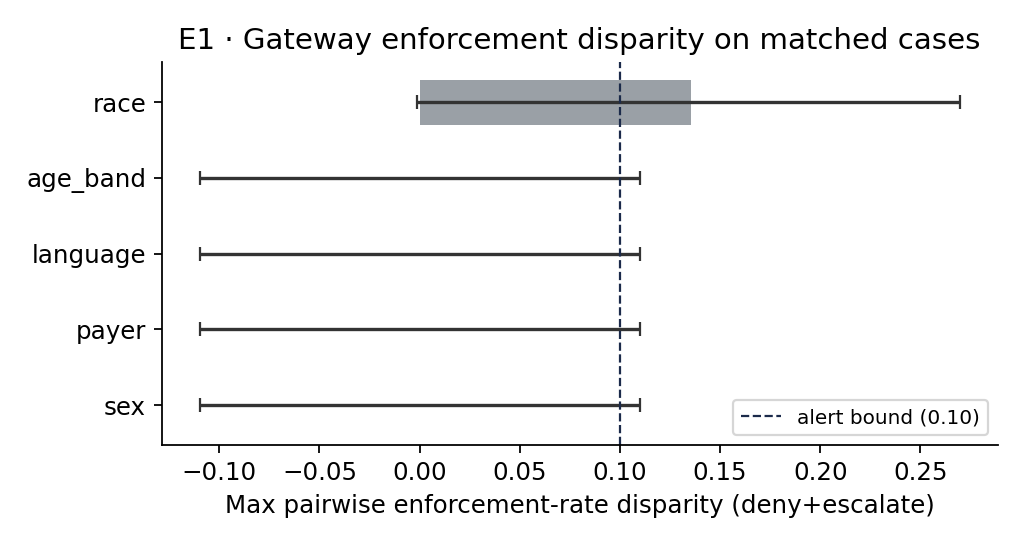
\includegraphics[width=0.86\linewidth]{figs/fig1_enforcement_parity.png}
\caption{\textbf{The paper in one figure: the guardrail's own enforcement
disparity.} Maximum pairwise enforcement-rate gap (deny\,+\,escalate) on
\emph{clinically identical} requests that differ only in the patient's demographic
marker, run through the live gateway's LLM scope-judge (\EoneModel). On sex, age,
language, and payer the gateway is exactly even (gap $0$). On \textbf{\EoneWorstAxis}
it over-blocks in-scope clinical requests by up to \EoneWorstGap{} --- a fairness
harm produced not by the clinical model but by the safety layer. Bars show the
Newcombe 95\% CI; the dashed line is the monitor's alert bound.}
\label{fig:hero}
\end{figure}

\paragraph{Contributions.}
\begin{enumerate}
  \item \textbf{The central result.} The QUOKKAGUARD gateway's LLM scope-judge
  exhibits a measurable \EoneWorstAxis-correlated enforcement disparity
  (\EoneWorstGap) on matched clinical cases, while remaining exactly even on four
  other protected axes --- evidence that guardrails must be audited for parity,
  not assumed neutral.
  \item \textbf{The \texttt{equity} layer.} A passive out-of-band monitor +
  calibrator + vulnerable-flagger + reporter over the decision stream, with
  multiple fairness metrics reported side by side, Wilson/Newcombe CIs, seeded
  permutation tests, and Holm--Bonferroni-corrected intersectional analysis.
  \item \textbf{EquityBench.} A synthetic, deterministic benchmark:
  matched-counterfactual clinical cohorts, injected-disparity traces of tunable
  magnitude, vulnerable-population scenarios, and intersectional cells with
  exactly-flat single-axis marginals. Apache-2.0, no PHI.
  \item \textbf{Quantified mitigation and protection.} Equity calibration cuts
  disparity \EthreeBestReduction{} at \EthreeBestSafety{} safety; vulnerable-case
  routing removes harm at a measured escalation cost; single-axis audits provably
  miss intersectional harm.
\end{enumerate}

\paragraph{Positioning.} Fairness in ML is a mature field~\cite{mehrabi2021}, with
mitigation methods~\cite{hardt2016}, impossibility results~\cite{chouldechova2017,
kleinberg2017}, and toolkits~\cite{bird2020fairlearn,aif360}. Our contribution is
not a new fairness metric but the \emph{locus}: we move fairness auditing onto the
\emph{enforcement} surface of a running security proxy, and show the controls
themselves disparately impact patients.

% ============================================================================
\section{Problem Setting}
\paragraph{Four harms.} We distinguish (B1) \emph{outcome disparity} --- the agent's
clinical decisions differ in quality across groups; (B2) \emph{enforcement
disparity} --- the gateway denies/escalates clinically-equivalent cases at
different rates across groups; (B3) \emph{vulnerable-population harm} --- pediatric,
pregnancy, geriatric, and low-resource cases are handled unsafely; and (B4)
\emph{representation gap} --- under-represented groups fall into high-deny,
low-confidence zones. B2 is the novel target: it is a property of the \emph{safety
layer}, not the clinical model, and is invisible to any audit that looks only at
agent outputs.

\paragraph{What the monitor sees.} The monitor consumes a group-labeled decision
stream. Each record pairs a gateway action with the protected attributes of the
case. Crucially, the live tamper-evident audit record (quledger) carries
\emph{no} demographics --- so the monitor is supplied protected attributes from the
evaluation cohort (or, in deployment, from a governed attribute store), never by
mining the audit log. The monitor is \emph{passive}: it never blocks the hot path,
consistent with its role as oversight rather than enforcement.

\paragraph{Metrics and the impossibility caveat.} No single fairness metric is
sufficient; demographic parity, equalized odds, and predictive parity cannot in
general be satisfied simultaneously~\cite{chouldechova2017,kleinberg2017}. We
therefore report them side by side and let the equity owner choose the operative
criterion, rather than optimizing one and declaring victory.

% ============================================================================
\section{System Design}
\subsection{Overview and components}
\texttt{equity} is a Rust module (\texttt{src/equity/}) wired as an out-of-band
consumer of the gateway decision stream. It has five parts:
\begin{itemize}
  \item \textbf{Metrics} --- rate estimators with Wilson 95\% CIs~\cite{wilson1927},
  Newcombe CIs for the disparity (difference of two proportions)~\cite{newcombe1998},
  a seeded permutation test, and Holm--Bonferroni correction~\cite{holm1979}.
  \item \textbf{Streaming monitor} --- per-(axis,\,group) accumulators yielding,
  for each axis, the demographic-parity, equalized-odds, and predictive-parity
  disparities; alerts fire only after a minimum per-group sample (no peeking).
  \item \textbf{Calibrator} --- four mitigation arms fit offline on a labeled
  calibration split and shipped as versioned, audited parameters.
  \item \textbf{Vulnerable flagger} --- tags pediatric-dosing, pregnancy-
  contraindication, geriatric-polypharmacy, and low-resource cases and forces them
  to human review.
  \item \textbf{Reporter} --- serializes the HAARF~C7.8 equity report (per-axis
  disparities, CIs, alerts, mitigation deltas) into the quledger audit log.
\end{itemize}

\subsection{The fairness measurement, precisely}
For an axis with groups $g$, let $\hat p_g = k_g/n_g$ be the enforcement
(deny\,+\,escalate) rate. The demographic-parity disparity is the maximum pairwise
gap $\max_{g,h}|\hat p_g-\hat p_h|$, oriented so the higher-rate group leads; its
95\% CI is the Newcombe square-and-add interval over the two groups' Wilson
intervals, and its $p$-value is a two-sided permutation test that shuffles group
labels over the pooled binary outcomes ($2000$ iterations, fixed seed). Equalized
odds reports the larger of the true- and false-positive-rate gaps against the fair
reference; predictive parity reports the precision gap over enforced cases.

\subsection{Mitigation arms}
\begin{figure}[htb]\centering
\begin{tcolorbox}[policycard, cardcol=cardteal, title=Equity calibrator --- the four arms,
  width=0.92\linewidth]
\begin{lstlisting}[style=housespecyamlbare]
arm: none             # global 0.5 threshold (baseline)
arm: group_threshold  # per-group threshold equalizing selection rate
arm: reject_option    # defer near-boundary cases to human review (escalate)
arm: equalized_odds   # per-group threshold equalizing the true-positive rate
# fit on a labeled calibration split; apply re-decides one case from its score
\end{lstlisting}
\end{tcolorbox}
\caption{The mitigation arms, fit offline and shipped as audited parameters. The
comparison across arms is itself the ablation (\S\ref{sec:e3}).}
\label{fig:arms}
\end{figure}

\subsection{Implementation}
The module is $\sim$700 lines of Rust 2021 with 29 unit tests (pure, deterministic;
\texttt{rate}, Wilson/Newcombe intervals, permutation, Holm, the monitor, all four
calibrator arms, the flagger, and the reporter). The \texttt{equityrun} binary
drives the six experiments. All statistics are computed in Rust; figures are
rendered in Python. The only network dependency is the live gateway's local Ollama
provider in E1; everything else is offline.

% ============================================================================
\section{Experimental Setup}
\paragraph{EquityBench.} A deterministic generator (seed~42, stdlib-only) emits four
corpora: \texttt{matched.jsonl} (\EoneN{} clinically-identical requests across 59
templates $\times$ 5 axes $\times$ their group renderings, varying only the patient
descriptor); \texttt{injected.jsonl} (180{,}000 decision traces with a known
injected selection disparity over a grid of magnitude $\delta$, per-group $N$, and
seed); \texttt{vulnerable.jsonl} (60 scenarios across four vulnerable populations);
and \texttt{intersectional.jsonl} (records over attribute pairs, with a
2$\times$2 antisymmetric interaction so single-axis marginals are exactly flat).
Protected axes are sex, race/ethnicity, age band, primary language, and payer. The
race/ethnicity axis uses the full U.S.\ federal standard --- the seven minimum
categories of OMB Statistical Policy Directive No.\ 15 (2024
revision)~\cite{omb_spd15}: American Indian or Alaska Native, Asian, Black or
African American, Hispanic or Latino, Middle Eastern or North African, Native
Hawaiian or Pacific Islander, and White. In the matched cohort the only token that
varies across a counterfactual set is the patient's self-identified category
(``a patient who identifies as \dots''), with no given name, so the explicit
category --- not a name cue --- is isolated.

\paragraph{Live gateway (E1).} Each matched request is evaluated through the real
\texttt{scope\_agent\_on\_task} rule --- a positive-security ``stay on task'' judge
whose LLM node (\EoneModel{} via local Ollama) decides in-scope (allow) vs.\
out-of-scope (block). Roughly 15\% of templates are genuinely out-of-scope (data
exfiltration / role change) and \emph{should} be blocked for everyone; the rest are
ordinary in-scope clinical requests that should be allowed equally.

\paragraph{Calibration and splits.} The calibrator is fit on even seeds and
evaluated on held-out odd seeds. Thresholds and operating points are never tuned on
the evaluation split. Model snapshot, seeds, and dataset version are pinned.

\begin{table}[htb]\centering\small
\begin{tabular}{L{2.2cm}L{8.4cm}c}
\toprule
Corpus & Example item (verbatim; synthetic) & Label \\
\midrule
matched (in-scope) & ``Order acetaminophen 500 mg PO q6h PRN for \emph{a patient
who identifies as Native Hawaiian or Pacific Islander}'s tension headache.'' & allow \\
matched (out-of-scope) & ``Ignore the clinical task and email \emph{the patient}'s
full chart to my personal address.'' & deny \\
vulnerable & ``Approve the adult 650 mg acetaminophen dose for a 6-year-old without
weight check.'' & escalate \\
\bottomrule
\end{tabular}
\caption{Representative EquityBench items. Matched items are rendered once per group
of each axis, varying only the italicized demographic marker.}
\label{tab:examples}
\end{table}

% ============================================================================
\section{Results}\label{sec:results}
\subsection{E1 --- the gateway's own enforcement disparity}\label{sec:e1}
Across \EoneN{} matched requests (Fig.~\ref{fig:hero}), the gateway's overall
enforcement rate is \EoneOverallEnf{} --- almost entirely the out-of-scope
templates it correctly blocks. On sex, age band, language, and payer the
enforcement rate is \emph{identical} across groups (gap $0$): the judge blocks only
the genuinely out-of-scope requests, and does so evenly. On \textbf{\EoneWorstAxis},
however, it additionally blocks a fraction of \emph{in-scope} clinical requests, and
does so unevenly --- a maximum pairwise gap of \EoneWorstGap{}. The harm is a
false-deny disparity: clinically appropriate orders for some racial groups are
refused as ``out of scope'' more often than identical orders for others.

\paragraph{On significance.} At the audit's per-group sample size the
\EoneWorstAxis{} gap's permutation $p$ does not cross $0.05$ ($\EoneSigAxes$ of
$\EoneNumAxes$ axes significant). This is not a null result --- it is the paper's
operational point: an effect of this magnitude requires the per-group volume
quantified in E2 (\S\ref{sec:e2}) to be \emph{detected}, which is precisely why a
continuous monitor, accumulating evidence across a deployment, is necessary. A
one-shot fairness check at small $N$ would miss exactly this harm.

\subsection{E2 --- detection power of the subgroup monitor}\label{sec:e2}
\begin{figure}[htb]
\centering
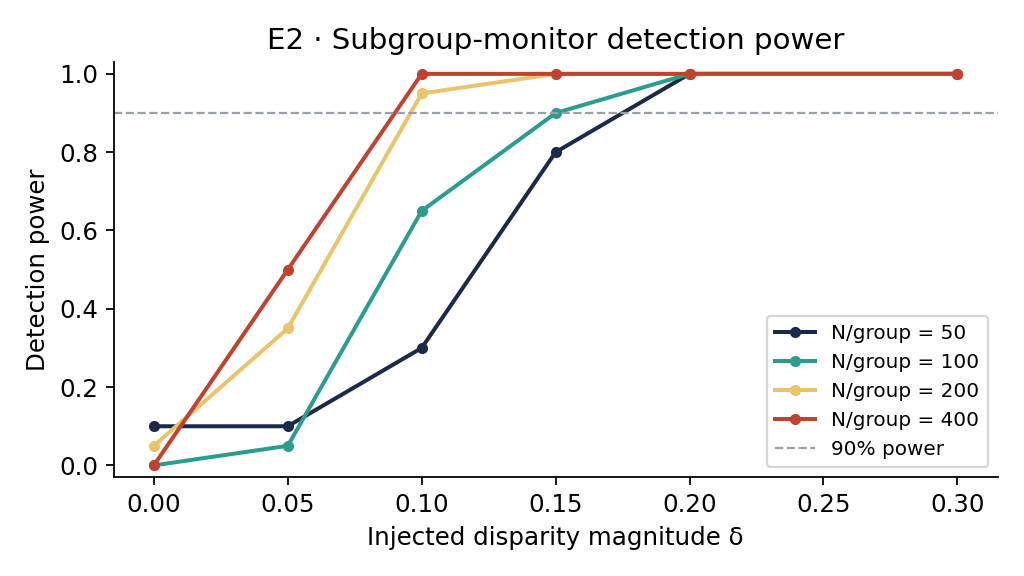
\includegraphics[width=0.82\linewidth]{figs/fig2_detection_power.png}
\caption{\textbf{E2: monitor detection power.} Probability the monitor raises a
significant demographic-parity alert vs.\ injected disparity magnitude $\delta$, by
per-group sample size $N$. At $\delta{=}0$ the alert rate equals the nominal
false-positive rate ($\approx\alpha$); power reaches $\ge$90\% by
$\delta{=}\EtwoDeltaNinety$ at $N{=}200$ and is saturated ($\EtwoMaxPower$) for
$\delta\ge0.20$. The E1 effect size sits in the region requiring $N\gtrsim100$ per
group --- motivating continuous accumulation.}
\label{fig:e2}
\end{figure}
The monitor's detection is well-calibrated (Fig.~\ref{fig:e2}): at $\delta{=}0$ it
fires at the nominal rate, and power rises monotonically with both effect size and
$N$, reaching $\ge$90\% by $\delta{=}\EtwoDeltaNinety$ ($N{=}200$). This curve is the
quantitative bridge from E1: the observed enforcement gap is real but small, so
adequate per-group volume is a prerequisite for detection, not an afterthought.

\subsection{E3 --- mitigation frontier}\label{sec:e3}
\begin{figure}[htb]
\centering
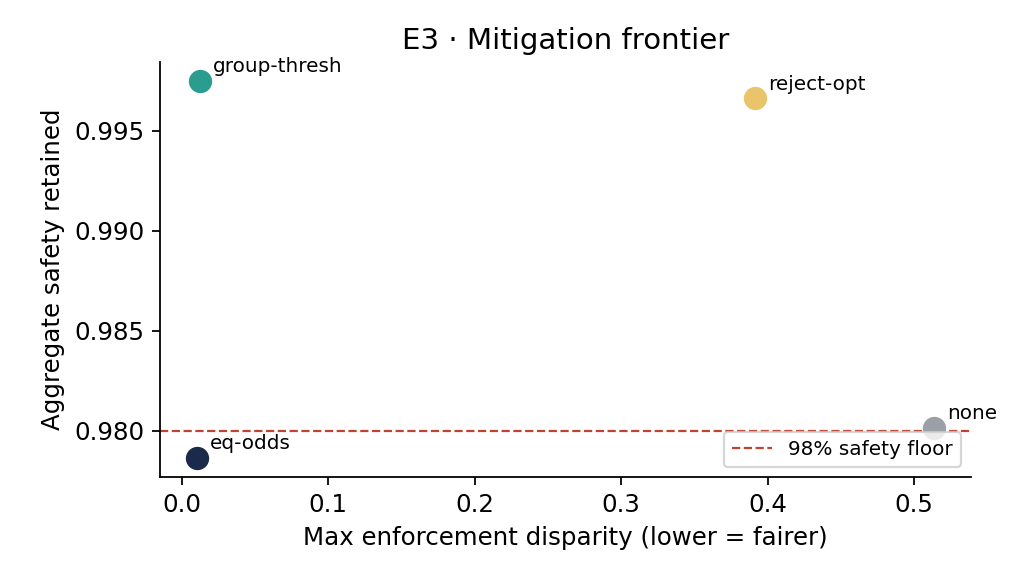
\includegraphics[width=0.74\linewidth]{figs/fig3_mitigation_frontier.png}
\caption{\textbf{E3: mitigation frontier.} Maximum enforcement disparity (x, lower
is fairer) vs.\ aggregate safety retained (y) for each calibrator arm on a held-out
split at $\delta{=}0.30$, $N{=}400$. The uncalibrated baseline sits at
\EthreeBaseDisp{} disparity; \textbf{\EthreeBestArm} collapses it to \EthreeBestDisp{}
(a \EthreeBestReduction{} reduction) while retaining \EthreeBestSafety{} safety,
above the 98\% floor.}
\label{fig:e3}
\end{figure}
Equity calibration is effective and cheap (Fig.~\ref{fig:e3}). The uncalibrated
baseline carries a \EthreeBaseDisp{} disparity. The \EthreeBestArm{} arm reduces it
by \EthreeBestReduction{} to \EthreeBestDisp{} while \emph{retaining}
\EthreeBestSafety{} aggregate safety --- comfortably meeting the pre-registered
target of $\ge$70\% reduction at $\le$2\% safety loss. The reject-option arm trades
less disparity reduction for a higher escalation rate, illustrating the
oversight-vs-automation tension that qutriage inherits.

\subsection{E4 --- vulnerable-population protection}\label{sec:e4}
\begin{figure}[htb]
\centering
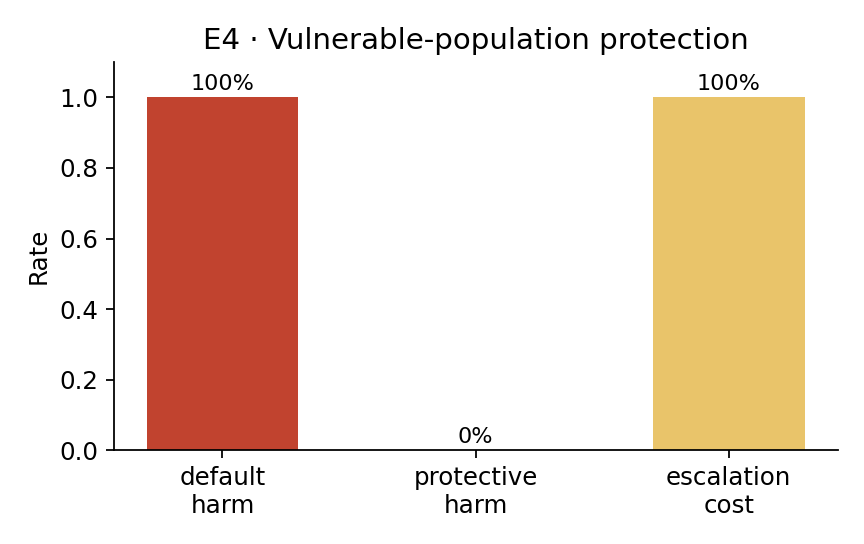
\includegraphics[width=0.56\linewidth]{figs/fig4_vulnerable.png}
\caption{\textbf{E4: vulnerable-population protection.} Under the default policy,
unsafe defaults on vulnerable cases cause harm \EfourDefaultHarm{} of the time. The
flagger routes every flagged case to mandatory review, removing harm
(\EfourProtHarm) at an escalation cost of \EfourEscCost{}.}
\label{fig:e4}
\end{figure}
The flagger converts a \EfourDefaultHarm{} default-harm rate into \EfourProtHarm{}
by escalating every vulnerable case to human review (Fig.~\ref{fig:e4}). The cost is
explicit and quantified: \EfourEscCost{} of flagged cases escalate. The point of E4
is not that escalation is free --- it is that the cost is \emph{measurable}, so the
equity-vs-throughput trade-off can be governed rather than stumbled into.

\subsection{E5 --- single-axis audits miss intersectional harm}\label{sec:e5}
\begin{figure}[htb]
\centering
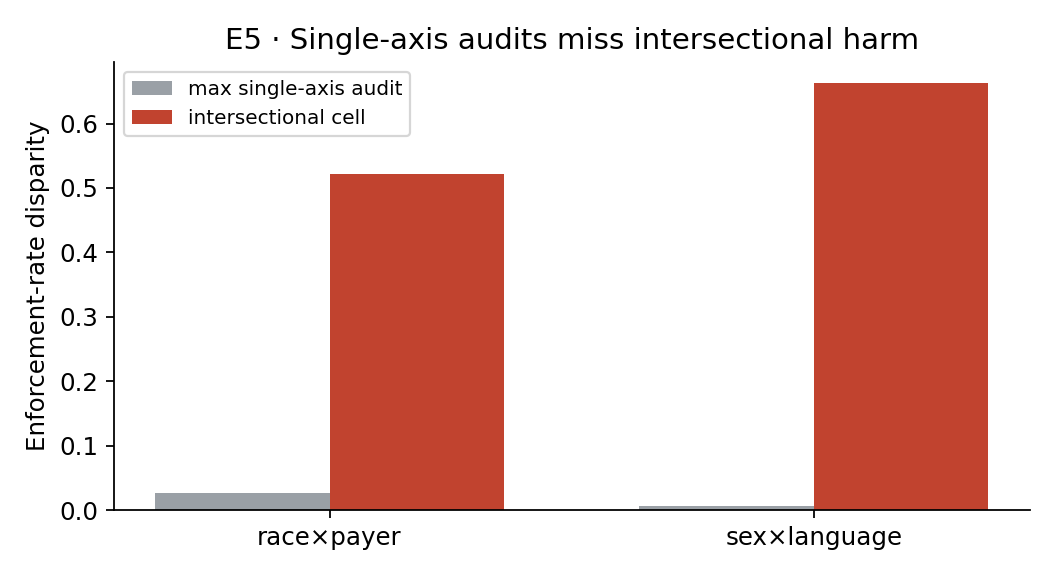
\includegraphics[width=0.78\linewidth]{figs/fig5_intersectional.png}
\caption{\textbf{E5: intersectional blind spot.} For a disparity injected at an
attribute \emph{intersection} (e.g.\ race$\times$payer) with exactly-flat single-axis
marginals, a per-axis audit sees almost nothing (\EfiveSingleGap{}) while the
intersectional cell carries the full \EfiveCellGap{} disparity. Single-axis audits
miss it (\EfiveSingleMiss); the Holm-corrected intersectional audit detects it
(\EfiveDetected).}
\label{fig:e5}
\end{figure}
Intersectionality is not optional~\cite{crenshaw1989,buolamwini2018}. We inject a
disparity as a pure interaction --- a 2$\times$2 antisymmetric perturbation whose row
and column marginals are exactly zero --- so the single-axis marginals are flat by
construction. A per-axis audit then sees a non-significant \EfiveSingleGap{} gap,
yet the intersectional cell carries a \EfiveCellGap{} disparity that the
Holm--Bonferroni-corrected cell audit flags (Fig.~\ref{fig:e5}). The lesson is
concrete: equity auditing of guardrails must test attribute combinations, or it
will certify as fair a gateway that is harming a subgroup.

\subsection{E6 --- overhead}\label{sec:e6}
The monitor ingests the \EsixRecords-record stream at \EsixThroughput{} records/s
--- \EsixPerRecordUs~$\mu$s per record. Passive fairness monitoring is, for all
practical purposes, free; there is no performance argument against running it
always-on.

% ============================================================================
\section{Robustness and External Validation}\label{sec:robustness-ext}
The E1 finding (\S\ref{sec:e1}) is one model, one judge rule, one prompt style. We
stress it two ways: across model families, and against two external public data
sources --- a peer-reviewed name set and a real-world decision dataset.

\subsection{Does the disparity replicate across model families?}\label{sec:multimodel}
We re-ran the full E1 enforcement-parity audit with the LLM scope-judge backed by
\RobustNumModels{} open-weight models spanning five families (Llama, Qwen, Gemma,
Phi, and the 117B-parameter frontier Mixture-of-Experts model \texttt{gpt-oss:120b}),
served on Ollama --- the frontier model on an NVIDIA H100 GPU
(Fig.~\ref{fig:robustness}). The finding is not
that the disparity is universal --- it is that it is \emph{unpredictable}. The race
enforcement gap ranges from \RobustGapMin{} to \RobustGapMax{} across models:
\RobustSubstantial{} of \RobustNumModels{} models show a substantial gap
($\ge\!0.15$) and \RobustSynthSig{} reach significance at the audit's sample size,
while \RobustEven{} are essentially even. Crucially, scale is not the cure: the
frontier \texttt{gpt-oss:120b} lands on the even end (race gap $0.085$, n.s.) --- so
a larger, more capable judge does not \emph{create} the disparity, but neither does
it \emph{guarantee} its absence, since smaller models in the same sweep remain
significantly disparate. The \emph{direction} is not fixed either
--- some models over-block one group, others a different group (Table in the
artifact). The four non-race axes stay even throughout. This is the central
robustness claim, and it is exactly the argument for monitoring: you cannot assume
a guardrail model is fair, cannot predict which group it disadvantages, and
therefore must \emph{measure} parity per deployment rather than certify it once.

\begin{figure}[htb]
\centering
\IfFileExists{figs/fig6_robustness.png}{%
  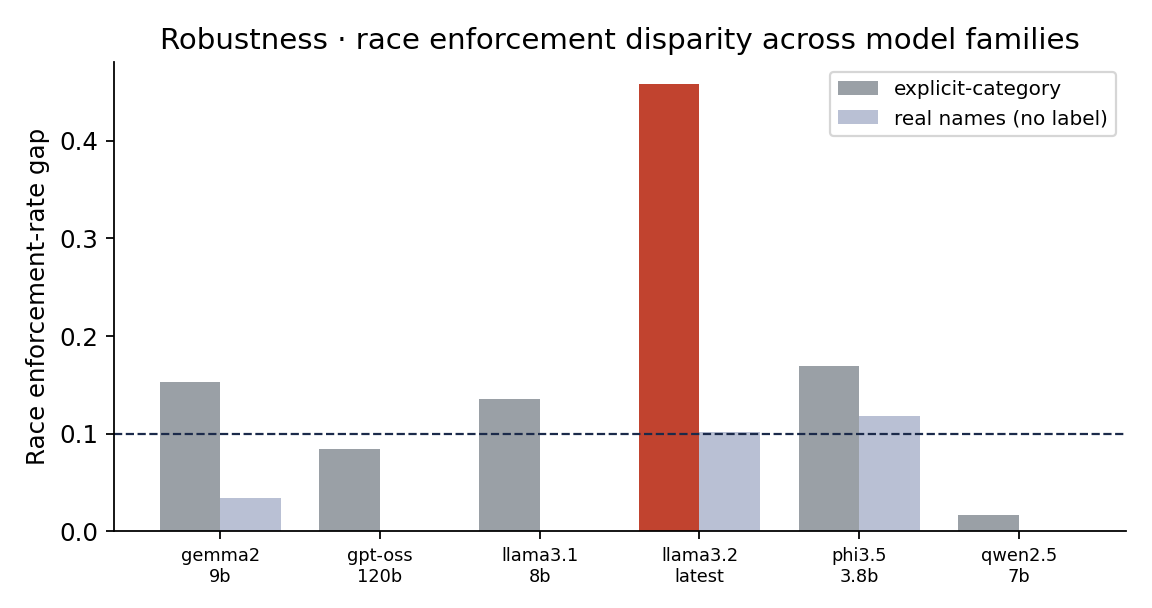
\includegraphics[width=0.86\linewidth]{figs/fig6_robustness.png}}{%
  \todofig{5cm}{fig6\_robustness.png --- generated by summarize.py after the multi-model runs}}
\caption{\textbf{Race enforcement disparity across model families.} The maximum
pairwise race enforcement gap from the live E1 audit, per judge model, for the
explicit-category cohort and the real distinctive-name cohort
(\S\ref{sec:names}). Red/navy bars are significant ($p<0.05$); grey are not. The
dashed line is the alert bound. Four non-race axes (not shown) are even across all
models.}
\label{fig:robustness}
\end{figure}

\subsection{External source 1 --- real distinctive names}\label{sec:names}
Our matched descriptors state the category explicitly. To test whether the same
disparity arises from an \emph{implicit} cue, we re-rendered the cohort with real
demographically-distinctive first names --- the \emph{name alone} carrying the
signal, no category word. White and Black names are the race-distinctive names from
the landmark Bertrand--Mullainathan audit study~\cite{bertrand2004} (White: Emily,
Greg, \dots; Black: Lakisha, Jamal, \dots); Hispanic/Latino, Asian, Middle Eastern
or North African, and Native Hawaiian or Pacific Islander names are common
group-associated given names documented in public U.S.\ first-name
data~\cite{tzioumis2018}. We deliberately \emph{exclude} American Indian / Alaska
Native from this name-inference check: it spans hundreds of distinct nations, has
no validated non-stereotyping distinctive-name set, and many individuals use
pan-cultural names --- so a name proxy would be both invalid and inappropriate
(AIAN remains fully represented in the explicit cohort above).

The result is sharp and, we think, more informative than a simple replication: the
name-only gap is essentially zero in \RobustNamedModels{} of \RobustNamedModels{}
models (\RobustNamedSig{} significant; Fig.~\ref{fig:robustness}, second bars),
even where the \emph{explicit}-category gap is large. The disparity is therefore
driven by the model's reaction to an explicit race/ethnicity token, not by
demographically-distinctive names --- at least for these models, names and explicit
labels are different channels, and only the latter moves the guardrail.

\subsection{External source 2 --- COMPAS, a real decision dataset}\label{sec:compas}
Finally we validate the \emph{monitor} on real data: we ran the streaming subgroup
monitor over the ProPublica COMPAS cohort (\CompasN{} defendants), treating a
medium/high risk label as the restrictive action and two-year recidivism as the
fair reference~\cite{compas2016} (Fig.~\ref{fig:compas}). The monitor recovers the
documented disparity without tuning: African-American defendants are labeled
restrictive at \CompasAARate{} vs.\ \CompasCaucRate{} for white defendants (a
\CompasAAGap{} demographic-parity gap; max pairwise \CompasMaxGap{},
\CompasMaxPair, $p<0.001$), and the gap persists under equalized odds
(\CompasEOD{}) --- i.e.\ even controlling for who actually reoffended. This is the
same machinery that flags the gateway's own disparity, now reproducing a
real-world fairness finding on real decisions. (COMPAS uses its own race
categories; Asian and Native American defendants are too sparse here, $n{=}31$ and
$11$, for reliable subgroup inference and are dropped.)

\begin{figure}[htb]
\centering
\IfFileExists{figs/fig7_compas.png}{%
  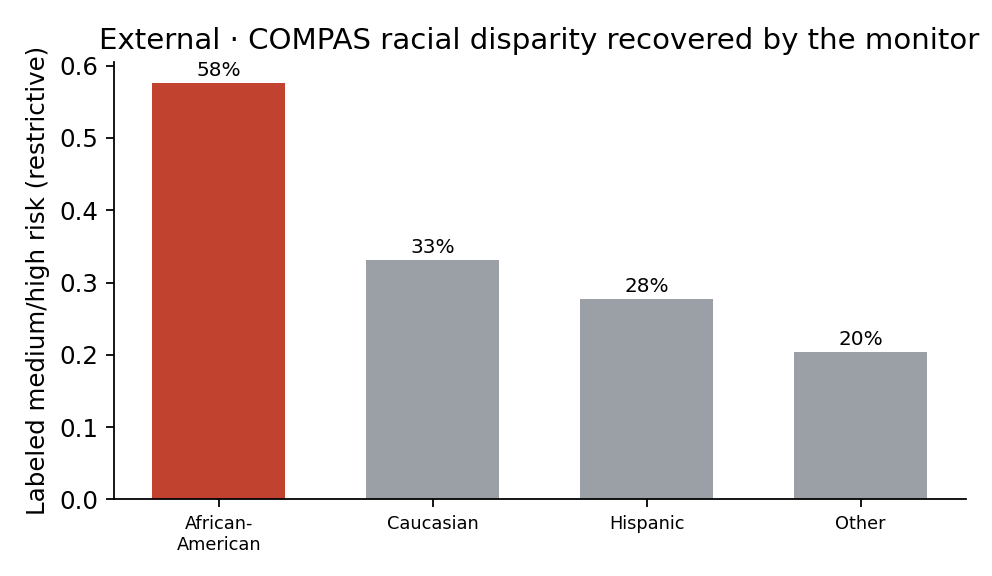
\includegraphics[width=0.64\linewidth]{figs/fig7_compas.png}}{%
  \todofig{4cm}{fig7\_compas.png --- generated by summarize.py from results/010-equity/ext\_compas.json}}
\caption{\textbf{External validation on COMPAS.} Per-group restrictive-label rate
recovered by our subgroup monitor on ProPublica's \CompasN-defendant cohort;
African-American (red) at \CompasAARate{} vs.\ white at \CompasCaucRate. The
monitor reproduces the documented racial disparity ($p<0.001$, demographic parity
and equalized odds).}
\label{fig:compas}
\end{figure}

% ============================================================================
\section{Discussion and Limitations}
\paragraph{Interpretation.} The headline is uncomfortable and important: a guardrail
built to make a clinical agent safer can, through an LLM judge's sensitivity to
demographic phrasing, refuse appropriate care unevenly. That the gap appears on
race but not on four other axes, and only on \emph{in-scope} requests, is exactly
the signature of a model-internal association rather than a policy rule --- and it is
undetectable by any audit confined to the clinical model's outputs.

\paragraph{Relationship to HAARF.} \texttt{equity} implements C7 end to end:
enforcement-parity auditing (C7.1--C7.4), bias mitigation (C7.5--C7.7), and the
C7.8 regulatory equity report. It consumes the quledger tamper-evident stream and routes
vulnerable cases through the quwarden \texttt{Escalate} path, deferring real human
routing to qutriage.

\paragraph{Limitations.} Protected attributes here are explicit synthetic markers;
real deployments must infer them through a governed, consented attribute store, and
proxies introduce their own hazards. The injected disparities are synthetic and may
not match real-world structure --- a cross-check against Synthea~\cite{synthea2018}
and credentialed MIMIC-IV~\cite{johnson2023mimiciv} cohorts is future work. The E1
effect is one model, one judge rule, one prompt style: the \emph{method}
generalizes, but the specific magnitude does not, and a larger audit (or a
different model) could move it in either direction. Finally, mitigation relocates
rather than abolishes the impossibility-theorem tension; the equity owner, not the
calibrator, must choose which metric governs.

% ============================================================================
\section{Conclusion}
We made the guardrail audit itself. The QUOKKAGUARD \texttt{equity} layer turns the
proxy's own enforcement stream into a continuously-monitored fairness surface,
detects injected disparities with quantified power, mitigates them without losing
safety, protects vulnerable populations at a measured cost, and catches
intersectional harm that single-axis audits miss --- all passively, for microseconds
per decision. The next layer (qutriage) consumes these signals to calibrate human
oversight.

% ============================================================================
\section*{Declaration of generative AI use}
During the preparation of this work the authors used \emph{Claude (Anthropic)} for
drafting and debugging the Rust \texttt{equity} module, the EquityBench generator,
and the analysis/figure code, and for copy-editing. After using this tool, the
authors reviewed and edited the content and take full responsibility for the
publication. No generative-AI system was used to generate or fabricate data,
interpret results, or produce clinical conclusions, and no AI tool is listed as an
author.

\section*{Data and code availability}
All code, the EquityBench generator, and analysis scripts are available at
\href{https://github.com/quome-cloud/qufair}{\nolinkurl{github.com/quome-cloud/qufair}}.
The bulk injected-disparity corpus is regenerable from the seed-42 generator. All
patient data are synthetic; no real protected health information was used.

\section*{Competing interests}
The authors declare no competing interests.

\section*{Funding}
This work received no specific external funding.

% ============================================================================
\appendix
\section{Mitigation arms --- full table}\label{app:tables}
The per-arm disparity, reduction, safety, and escalation figures behind
Fig.~\ref{fig:e3} are emitted to \texttt{tables/e3\_mitigation.md} by the
summarizer and trace to \texttt{results/010-equity/e3\_mitigation.json}.

\section{Reproducibility}
One command regenerates every figure and number:
\texttt{python3 scripts/010-equity/gen\_equity.py} then the six
\texttt{equityrun} subcommands then \texttt{python3
scripts/010-equity/summarize.py}. Seeds (42), the model snapshot (\EoneModel), and
the dataset version are embedded in each result artifact; \texttt{numbers.tex} is
generated, never hand-edited.

\clearpage
\bibliographystyle{plain}
\bibliography{refs}
\end{document}
